% Created 2018-04-09 Mon 22:33
% Intended LaTeX compiler: pdflatex
\documentclass[11pt]{article}
\usepackage[utf8]{inputenc}
\usepackage[T1]{fontenc}
\usepackage{graphicx}
\usepackage{grffile}
\usepackage{longtable}
\usepackage{wrapfig}
\usepackage{rotating}
\usepackage[normalem]{ulem}
\usepackage{amsmath}
\usepackage{textcomp}
\usepackage{amssymb}
\usepackage{capt-of}
\usepackage{hyperref}
\usepackage{amssymb}
\usepackage{color}
\usepackage{istgame}
\date{\today}
\title{}
\hypersetup{
 pdfauthor={},
 pdftitle={},
 pdfkeywords={},
 pdfsubject={},
 pdfcreator={Emacs 26.0.91 (Org mode 9.1.6)}, 
 pdflang={English}}
\begin{document}

\tableofcontents


\section{Spieltheorie}
\label{sec:org279dffd}
In der Spieltheorie gibt es im Unterschied zur Entscheidungstheorie eine \textbf{Bimatrix} statt der Auszahlungsmatrix. In dieser sind die Einträge bereits \emph{Nutzengrößen}. Die Unsicherheit existiert nun nicht mehr im Hinblick auf Umweltzustände, sondern im Hinblick auf die Strategie eines weiteren Spielers. Da man nun die Auszahlungen für beide Spieler angeben muss, benötigt man zwei Matrizen \emph{oder} eine mit doppelten Einträgen, also eine "Bimatrix".
\begin{center}
\begin{tabular}{c|c|c|c}
S & s\(^{\text{1}}_{\text{2}}\) & s\(^{\text{2}}_{\text{2}}\) & s\(^{\text{3}}_{\text{2}}\)\\
\hline
s\(^{\text{1}}_{\text{1}}\) & (u\(_{\text{1}}\)(s\(^{\text{1}}_{\text{1,s}}\)\(^{\text{1}}_{\text{2}}\)), u\(_{\text{2}}\)(s\(^{\text{1}}_{\text{1}}\), s\(^{\text{1}}_{\text{2}}\))) & (u\(_{\text{1}}\)(s\(^{\text{1}}_{\text{1,s}}\)\(^{\text{2}}_{\text{2}}\)), u\(_{\text{2}}\)(s\(^{\text{1}}_{\text{1}}\), s\(^{\text{2}}_{\text{2}}\))) & (u\(_{\text{1}}\)(s\(^{\text{1}}_{\text{1,s}}\)\(^{\text{3}}_{\text{2}}\)), u\(_{\text{2}}\)(s\(^{\text{1}}_{\text{1}}\), s\(^{\text{3}}_{\text{2}}\)))\\
s\(^{\text{2}}_{\text{1}}\) & (u\(_{\text{1}}\)(s\(^{\text{2}}_{\text{1,s}}\)\(^{\text{1}}_{\text{2}}\)), u\(_{\text{2}}\)(s\(^{\text{2}}_{\text{1}}\), s\(^{\text{1}}_{\text{2}}\))) & (u\(_{\text{1}}\)(s\(^{\text{2}}_{\text{1,s}}\)\(^{\text{2}}_{\text{2}}\)), u\(_{\text{2}}\)(s\(^{\text{2}}_{\text{1}}\), s\(^{\text{2}}_{\text{2}}\))) & (u\(_{\text{1}}\)(s\(^{\text{2}}_{\text{1,s}}\)\(^{\text{3}}_{\text{2}}\)), u\(_{\text{2}}\)(s\(^{\text{2}}_{\text{1}}\), s\(^{\text{3}}_{\text{2}}\)))\\
s\(^{\text{3}}_{\text{1}}\) & (u\(_{\text{1}}\)(s\(^{\text{3}}_{\text{1,s}}\)\(^{\text{1}}_{\text{2}}\)), u\(_{\text{2}}\)(s\(^{\text{3}}_{\text{1}}\), s\(^{\text{1}}_{\text{2}}\))) & (u\(_{\text{1}}\)(s\(^{\text{3}}_{\text{1,s}}\)\(^{\text{2}}_{\text{2}}\)), u\(_{\text{2}}\)(s\(^{\text{3}}_{\text{1}}\), s\(^{\text{2}}_{\text{2}}\))) & (u\(_{\text{1}}\)(s\(^{\text{3}}_{\text{1,s}}\)\(^{\text{3}}_{\text{2}}\)), u\(_{\text{2}}\)(s\(^{\text{3}}_{\text{1}}\), s\(^{\text{3}}_{\text{2}}\)))\\
\end{tabular}
\end{center}
Die Nummer der Strategie ist nun im Gegensatz zu Kapitel 1 hochgestellt, unten steht die Nummer des Spielers.
\subsection{Beispiele}
\label{sec:org52426ea}
\subsubsection{Hirschjagd}
\label{sec:org0895d08}
\begin{center}
\begin{tabular}{c|c|c}
\textcolor{magenta}{Jäger 1}/\textcolor{blue}{Jäger 2} & \textcolor{blue}{Hirsch} & \textcolor{blue}{Hase}\\
\hline
\textcolor{magenta}{Hirsch} & (\textcolor{magenta}{5},\textcolor{blue}{5}) & (\textcolor{magenta}{0},\textcolor{blue}{4})\\
\textcolor{magenta}{Hase} & (\textcolor{magenta}{4},\textcolor{blue}{0}) & (\textcolor{magenta}{4},\textcolor{blue}{4})\\
\end{tabular}
\end{center}
\subsubsection{Kopf oder Zahl}
\label{sec:org3129aa0}
Jeder Spieler legt unbeobachtbar für den anderen Spieler eine Münze, stimmen die Bilder überein erhält Spieler 1 die Münzen, unterscheiden sie sich so erhält Spieler 2 die Münzen.
\begin{center}
\begin{tabular}{c|c|c}
\textcolor{magenta}{Spieler 1}/\textcolor{blue}{Spieler 2} & \textcolor{blue}{Kopf} & \textcolor{blue}{Zahl}\\
\hline
\textcolor{magenta}{Kopf} & (\textcolor{magenta}{1},\textcolor{blue}{-1}) & (\textcolor{magenta}{-1},\textcolor{blue}{1})\\
\textcolor{magenta}{Zahl} & (\textcolor{magenta}{-1},\textcolor{blue}{1}) & (\textcolor{magenta}{1},\textcolor{blue}{-1})\\
\end{tabular}
\end{center}
Ist ein Nullsummenspiel da \(E(\pi) = 0\)
\subsubsection{Kampf der Geschlechter}
\label{sec:org5bd2051}
\begin{center}
\begin{tabular}{c|c|c}
\textcolor{magenta}{Sie}/\textcolor{blue}{Er} & \textcolor{blue}{Theater} & \textcolor{blue}{Fußball}\\
\hline
\textcolor{magenta}{Theater} & (\textcolor{magenta}{4},\textcolor{blue}{3}) & (\textcolor{magenta}{2},\textcolor{blue}{2})\\
\textcolor{magenta}{Fußball} & (\textcolor{magenta}{1},\textcolor{blue}{1}) & (\textcolor{magenta}{3},\textcolor{blue}{4})\\
\end{tabular}
\end{center}
\subsubsection{Chicken/Hasenfuss-Spiel}
\label{sec:orgdf0addd}
\begin{center}
\begin{tabular}{c|c|c}
\textcolor{magenta}{Fahrer 1}/\textcolor{blue}{Fahrer 2} & \textcolor{blue}{geradeaus} & \textcolor{blue}{ausweichen}\\
\hline
\textcolor{magenta}{geradeaus} & (\textcolor{magenta}{0},\textcolor{blue}{0}) & (\textcolor{magenta}{4},\textcolor{blue}{2})\\
\textcolor{magenta}{ausweichen} & (\textcolor{magenta}{2},\textcolor{blue}{4}) & (\textcolor{magenta}{3},\textcolor{blue}{3})\\
\end{tabular}
\end{center}
\subsubsection{Gefangenendilemma}
\label{sec:orgdc1e994}
\begin{center}
\begin{tabular}{c|c|c}
\textcolor{magenta}{Spieler 1}/\textcolor{blue}{Spieler 2} & \textcolor{blue}{schweigen} & \textcolor{blue}{gestehen}\\
\hline
\textcolor{magenta}{schweigen} & (\textcolor{magenta}{4},\textcolor{blue}{4}) & (\textcolor{magenta}{0},\textcolor{blue}{5})\\
\textcolor{magenta}{gestehen} & (\textcolor{magenta}{5},\textcolor{blue}{0}) & (\textcolor{magenta}{1},\textcolor{blue}{1})\\
\end{tabular}
\end{center}

Ein Spiel in strategischer Form ist ein Tripel: \(\Gamma = (I,(S_i)_{i \epsilon I} ,(u_i)_{i \epsilon I})\) \\
I = endliche, nichtleere Menge der Spieler zB: \{Unternehmen 1, Unternehmen 2\}\\
S = S\(_{\text{1}}\) x S\(_{\text{2}}\) x \ldots{} x S\(_{\text{i}}\) ist die Menge der Strategiekombinationen\\
S\(_{\text{i}}\) = die Strategiemenge jedes Spielers zB:

S\(_{\text{1}}\)=\{s\(^{\text{1}}_{\text{1}}\), s\(^{\text{2}}_{\text{1}}\)\}=\{Regenschirm, Sonnenschrim\}

S\(_{\text{2}}\)=\{s\(^{\text{1}}_{\text{2}}\), s\(^{\text{2}}_{\text{2}}\)\}=\{Sonnenschirm, Regenschirm\}

\(\rightarrow\) somit ist \(S = S_1 * S_2 = {(R,S), (R,R), (S,S), (S,R)}\) \\
u\(_{\text{i}}\) = die Auszahlungsfunktion eines jeden Spielers in Abhängigkeit von S zB für Spieler 1 von der Schirmproduktion:
\begin{center}
\begin{tabular}{ll}
\(u_1(R, S) = 10\) & \(u_1(R,R)=9\)\\
\(u_1(S, S) = 8\) & \(u_1(S,R)=11\)\\
\end{tabular}
\end{center}
und für Spieler 2:
\begin{center}
\begin{tabular}{ll}
\(u_2(R, S) = 5\) & \(u_2(R,R)=1\)\\
\(u_2(S, S) = 4\) & \(u_2(S,R)=2\)\\
\end{tabular}
\end{center}

\subsection{Beste Antworten}
\label{sec:orgbb459d5}
Sei S\(_{\text{i}}\) eine Menge von Strategien aller anderen Spieler außer Spieler i. Dann liefert die Beste-Antwort-Korrespondenz B\(_{\text{i}}\) die Menge aller Strategien von Spieler i, die potenziell beste Antworten sein könnten. Eine beste Antwort auf eine Strategie ist
die Menge aller optimalen Reaktionen. Wenn es mehrere mögl. gegnerische Strategien gibt, dann gibt es dementsprechend auch mehrere mögliche beste Antworten.

\paragraph{Beispiel Hirschjagd:}
\(B_1(Hirsch) = Hirsch\) und \(B_1(Hase)=Hase\) das bedeutet die beste Antwort auf die gegnerische Strategie "Hirsch" ist für Spieler 1 Hirsch und auf Hase lautet die beste Antwort Hase.\\
\(B_2(Hirsch) = Hirsch\) und \(B_2(Hase)=Hase\) das bedeutet die beste Antwort auf die gegnerische Strategie "Hirsch" ist für Spieler 2 Hirsch und auf Hase lautet die beste Antwort Hase. \\
Alle Beste Antworten Spieler 1: \(B_1(\{Hirsch,Hase\})=\{Hirsch, Hase\}\) \\
Alle Beste Antworten Spieler 2: \(B_1(\{Hirsch,Hase\})=\{Hirsch, Hase\}\) 

\paragraph{Beispiel Chicken}
\begin{equation*}
\begin{aligned}
B_1(\{geradeaus, ausweichen\})= \{ausweichen, geradeaus\} \\
B_2(\{geradeaus, ausweichen\})= \{ausweichen, geradeaus\}
\end{aligned}
\end{equation*}

\paragraph{Beispiel Schirmproduktion}
\begin{equation*}
\begin{aligned}
B_1(\{S, R\})=\{R, S\} \\
B_2(\{S, R\})=\{S, S\} 
\end{aligned}
\end{equation*}

\subsubsection{Dominanz}
\label{sec:orgc230106}
Eine Strategie s\(_{\text{i}}\) dominiert(schwach) eine andere Strategie s'\(_{\text{i}}\) falls s\(_{\text{i}}\) für \textbf{alle gegnerischen} Strategien einen \textbf{mindestens gleichhohen} Nutzen wie s'\(_{\text{i}}\) liefert, formal: \\
\begin{equation*}
\begin{aligned}
u_i(s_i, s_{-i}) \geq u_i(s'_i, s_{-i})
\end{aligned}
\end{equation*}
für alle s\(_{\text{-i}}\) \(\epsilon\) S\(_{\text{-i}}\) also alle gegnerischen Strategien. Von strenger Dominanz spricht man wenn statt \(\ge\) ">" gilt.

\paragraph{Dominanz beim Gefangenendilemma}
\begin{center}
\begin{tabular}{c|c|c}
\textcolor{magenta}{Spieler 1}/\textcolor{blue}{Spieler 2} & \textcolor{blue}{schweigen} & \textcolor{blue}{gestehen}\\
\hline
\textcolor{magenta}{schweigen} & (\textcolor{magenta}{4},\textcolor{blue}{4}) & (\textcolor{magenta}{0},\textcolor{blue}{5})\\
\textcolor{magenta}{gestehen} & (\textcolor{magenta}{5},\textcolor{blue}{0}) & (\textcolor{magenta}{1},\textcolor{blue}{1})\\
\end{tabular}
\end{center}

Für Spieler 2 wird "schweigen" dominiert, denn 5 > 4 und 1 > 0. Spieler 1 antizipiert, dass Spieler 2 keine dominierte Strategie (also nicht "schweigen"), sondern "gestehen" spielen wird. Somit muss sich Spieler 1 dann nur noch zwischen 0 und 1 entscheiden da s\(^{\text{1}}_{\text{2}}\) wegfällt. Er wird gestehen wählen weil 1 > 0.

\subsubsection{Beste Antworten auf Wahrscheinlichkeitsverteilungen}
\label{sec:orga016a67}
Angenommen die Gegenspieler haben gemischte Strategien. Dann liefert die Beste-Antwort-Korrespondenz B\(_{\text{i}}\) die Menge aller Beste-Antwort-Strategien. Es ändert sich eigentlich nichts, nur dass der Spieler i jetzt auf einen “unberechenbaren” Gegenspieler reagiert und die optimale Reaktion suchen muss.\\
Es werden also die besten Antworten auf Wahrscheinlichkeitsverteilungen gesucht:
\begin{center}
\begin{tabular}{c|c|c}
\textcolor{magenta}{Spieler 1}/\textcolor{blue}{Spieler 2} & \textcolor{blue}{Kopf}(\(\sigma_{\text{2}}\)) & \textcolor{blue}{Zahl}(1-\(\sigma_{\text{2}}\))\\
\hline
\textcolor{magenta}{Kopf}(\(\sigma_{\text{1}}\)) & (\textcolor{magenta}{1},\textcolor{blue}{-1}) & (\textcolor{magenta}{-1},\textcolor{blue}{1})\\
\textcolor{magenta}{Zahl}(1-\(\sigma_{\text{1}}\)) & (\textcolor{magenta}{-1},\textcolor{blue}{1}) & (\textcolor{magenta}{1},\textcolor{blue}{-1})\\
\end{tabular}
\end{center}
Erwarteter Nutzen Spieler 1:\\
\begin{equation*}
\begin{aligned}
u_i(\sigma_1,\sigma_2) = 1* \sigma_1* \sigma_2 + (-1) * \sigma_1 * (1- \sigma_2) + (-1)*(1- \sigma_1)* \sigma_2+1*(1-  \sigma_1)(1- \sigma_2)
\end{aligned}
\end{equation*}
Um herauszufinden wie Spieler 1 seinen Nutzen maximieren kann, muss diese Funktion partiel nach \(\sigma_{\text{1}}\) abgeleitet werden:\\
\begin{equation*}
\begin{aligned}
f'_{\sigma_1}=4 \sigma_2 - 2
\end{aligned}
\end{equation*}
wenn \(\sigma_2 = \frac{1}{2}\) ist, dann ist \(f'_{sigma_1}=0\) \(\rightarrow\) beste Antwort ist unbestimmt: \(\sigma_{\text{1}}\) \(\epsilon\) [0,1]\\
wenn \(\sigma_2 > \frac{1}{2}\) ist, dann ist \(f'_{sigma_1}>0\) \(\rightarrow\) beste Antwort ist \(\sigma_{\text{1}}\) = 100\% also ist BA die Wahl von Strategie s\(^{\text{1}}_{\text{1}}\)
wenn \(\sigma_2 < \frac{1}{2}\) ist, dann ist \(f'_{sigma_1}<0\) \(\rightarrow\) beste Antwort is \(\sigma_{\text{1}}\) = 0\% also ist BA die Wahl von Strategie s\(^{\text{2}}_{\text{1}}\)\\
\newpage
Beste Antwort von Spieler 1 auf Spieler \(\sigma_{\text{1}}\) in Abhängigkeit von \(\sigma_{\text{2}}\) sieht wie folgt aus:
\begin{figure}[htbp]
\centering
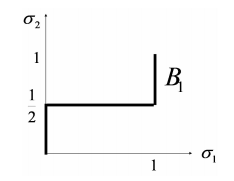
\includegraphics[width=100px]{./Kop_Zahl_BA.png}
\caption{Beste-Antworten beider Spieler 1}
\end{figure}
\subsection{Das Nash-Gleichgewicht}
\label{sec:org86be637}
\subsubsection{NashGG in reinen Strategien}
\label{sec:org9ca2f09}
Mit dem Nash-GG kann man die Menge der Antworten noch weiter einschränken als durch das Aussortieren dominierter Strategien (denn die Strategie eines Nash-GG) wird nie (strikt) dominiert.\\
S ist ja die Menge der Strategiekombinationen, darin enthalten zB \{Hase, Hase\} oder \{RS, SS\}. Als \(s^* = (s^*_1, s^*_2, s^*_3, s^*_4) \epsilon S\) wird dann ein Nash-GG(in reinen Strategien) gekennzeichnet, wenn für alle i \(\le\) n gilt \\
\begin{equation*}
\begin{aligned}
s^*_i \epsilon B_i(s^*_1)
\end{aligned}
\end{equation*}
Diese Formel besagt das s\(^{\text{*}}_{\text{i}}\), also die Strategie von Spieler i, in den optimalen Beste-Antworten auf alle Strategien der Gegenspieler also s\(^{\text{*}}_{\text{-i}}\) beinhaltet sein muss. Wenn dies für alle i also für alle Spieler der Fall ist, handelt es sich um ein NashGG. Zum Beispiel Nash-GG, in dem beide Jäger auf Hirsch gehen, denn:

\(B_{\textcolor{magenta}{1}}(\textcolor{blue}{Hirsch}) = \textcolor{magenta}{Hirsch}\)
und
\(B_{\textcolor{blue}{2}}(\textcolor{magenta}{Hirsch}) = \textcolor{blue}{Hirsch}\)

Wenn beide Jäger auf Hase gehen, ist das auch ein Nash-GG, denn:
\(B_{\textcolor{magenta}{1}}(\textcolor{blue}{Hase}) = \textcolor{magenta}{Hase}\)
und
\(B_{\textcolor{blue}{2}}(\textcolor{magenta}{Hase}) = \textcolor{blue}{Hase}\)

Die Strategiekombinationen (Hirsch,Hase) und (Hase, Hirsch) sind jedoch keine NashGGs.

\subsubsection{NashGG in gemischten Strategien}
\label{sec:org9f02174}
Gibt es bei dem Spiel Kopf oder Zahl etwa kein Gleichgewicht?! Wie bereits gelernt können auch gemischte Strategien beste Antworten sein und werden somit auch als NashGG zugelassen.
Siehte weiter oben:
\begin{center}
\begin{tabular}{c|c|c}
\textcolor{magenta}{Spieler 1}/\textcolor{blue}{Spieler 2} & \textcolor{blue}{Kopf}(\(\sigma_{\text{2}}\)) & \textcolor{blue}{Zahl}(1-\(\sigma_{\text{2}}\))\\
\hline
\textcolor{magenta}{Kopf}(\(\sigma_{\text{1}}\)) & (\textcolor{magenta}{1},\textcolor{blue}{-1}) & (\textcolor{magenta}{-1},\textcolor{blue}{1})\\
\textcolor{magenta}{Zahl}(1-\(\sigma_{\text{1}}\)) & (\textcolor{magenta}{-1},\textcolor{blue}{1}) & (\textcolor{magenta}{1},\textcolor{blue}{-1})\\
\end{tabular}
\end{center}

\[ B_1(\sigma_2) =\begin{cases} 
      0 & \sigma_2 < \frac{1}{2} \\
      [0;1] & \sigma_2 = \frac{1}{2} \\
      1 & \sigma_2 > \frac{1}{2} 
   \end{cases}
\]

\[ B_2(\sigma_1) =\begin{cases} 
      1 & \sigma_1 < \frac{1}{2} \\
      [0;1] & \sigma_1 = \frac{1}{2} \\
      0 & \sigma_1 > \frac{1}{2} 
   \end{cases}
\]
Was bedeutet das obige? Die Spieler 1,..,i wählen ihre erste Strategie mit der Wahrscheinlichkeit \(\sigma_{\text{i}}\) und dementsprechend die zweite mit der Wahrscheinlichkeit \(1 - \sigma_i\) . Da beide Spieler in Abhängigkeit von der Strategiewahl des jeweils anderen Spielers eine unterschiedlichen Nutzen erlangen, hängt ihre Beste-Antwort von der Wahrscheinlichkeit mit der der Gegenspieler seine Strategien wählt ab. Was bei B\(_{\text{i}}\) als erstes hinter der geschweiften Klammer steht ist also der optimale Wert für "Wahrscheinlichkeit" \(\sigma_{\text{i}}\) mit der man selber agieren sollte um den maximalen Nutzen zu erzielen. Das hängt vom jeweiligen Wert der Wahrscheinlichkeit des Gegenspielers ab.\\
Im obigen Beispiel ist die beste Antwort des ersten Spielers \(BA_1(\sigma_2)\) auf ein \(\sigma_2 < \frac{1}{2}\) (Wahrscheinlichkeit das Spieler 2 Kopf spielt) der Wert \textcolor{magenta}{0} für \(\textcolor{magenta}{\sigma_1}\), was wie man in der Tabelle sehen kann, bedeuten würde, dass er am besten Zahl spielt, denn \(\textcolor{magenta}{Zahl(1-\sigma_1)}\), also \(1-\textcolor{magenta}{0}\) = 100\% Wahrscheinlichkeit.
\begin{figure}[htbp]
\centering
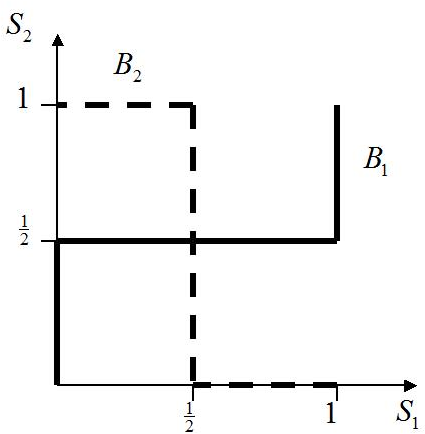
\includegraphics[width=100px]{./Kop_Zahl_BA2.png}
\caption{wechselseitig Beste-Antworten beider Spieler}
\end{figure}
\newline
NashGG's liegen dort, wo sich beide Funktionen schneiden in diesem Fall also bei \(\sigma_1=50\%\) , \(\sigma_2=50\%\) . Macht Sinn, denn bei anderer Wahrscheinlichkeit würde ein Spieler ja auch zu berechenbar werden. 

\paragraph{Polizeispiel}
\begin{center}
\begin{tabular}{c|c|c}
\textcolor{magenta}{Behörde}/\textcolor{blue}{Straftäter} & \textcolor{blue}{Betrug}(\(\sigma_{\text{2}}\)) & \textcolor{blue}{kein B.}(1-\(\sigma_{\text{2}}\))\\
\hline
\textcolor{magenta}{Kontrolle}(\(\sigma_{\text{1}}\)) & (\textcolor{magenta}{4-C},\textcolor{blue}{1-F}) & (\textcolor{magenta}{4-C},\textcolor{blue}{0})\\
\textcolor{magenta}{keine K.}(1-\(\sigma_{\text{1}}\)) & (\textcolor{magenta}{0},\textcolor{blue}{1}) & (\textcolor{magenta}{4},\textcolor{blue}{0})\\
\end{tabular}
\end{center}
In (Nash-)Gleichgewichten in gemischten Strategien sind alle Spieler indifferent zwischen den Handlungsalternativen.\\
Nutzen der Behörde bei Kontrolle: \(4-C\) \\
Nutzen der Behörde ohne Kontrolle: \(\sigma_2 * 0 + (1- \sigma_2)*4\) \\
Behörde also indifferent, wenn der Nutzen beider Strategien gleich ist:\\
\(4-C=\sigma_2 * 0 + (1- \sigma_2)*4\) \(\rightarrow\) Indifferent bei \(\sigma_2 = \frac{C}{4}\) .\\
\newline
Nutzen des Straftäters bei Betrug: \(\sigma_1 * (1-F) + (1-\sigma_1) * 1\) \\
Nutzen des Straftäters ohne Betrug: \(0\) \\
Straftäter also indifferent, wenn der Nutzen beider Strategien gleich ist:\\
\(\sigma_1 * (1-F) + (1-\sigma_1) * 1 = 0\) \(\rightarrow\) Indifferent bei \(\sigma_1 = \frac{1}{4}\)

\paragraph{Polizeispiel}
\textbf{Satz von Nash:} jedes endliche Spiel hat mind. ein GLeichgewicht, wenn man gemischte Strategien zulässt\\
\textbf{Satz von Wilson:} fast alle endlichen Spiele haben eine endliche, ungerade Anzahl von Gleichgewichten.
\subsection{Dynamische Spiele bei perfekter Information}
\label{sec:orgddfc6b6}
Annahme, dass perfekte Informationen (alle bisherigen Spielzüge bekannt) bekannt sind und keine Züge der Natur vorliegen (aber auch leicht erweiterbar auf Spiele mit Zügen der Natur)
\paragraph{Ultimatum-Spiel:}
\begin{itemize}
\item Aufteilung von drei Münzen zwischen zwei Spielern
\item Spieler 1 macht einen Vorschlag, Spieler 2 nimmt an oder lehnt ab
\item Bei Ablehnung bekommt keiner der Spieler etwas
\item Keine Nachverhandlungen
\end{itemize}
\begin{center}
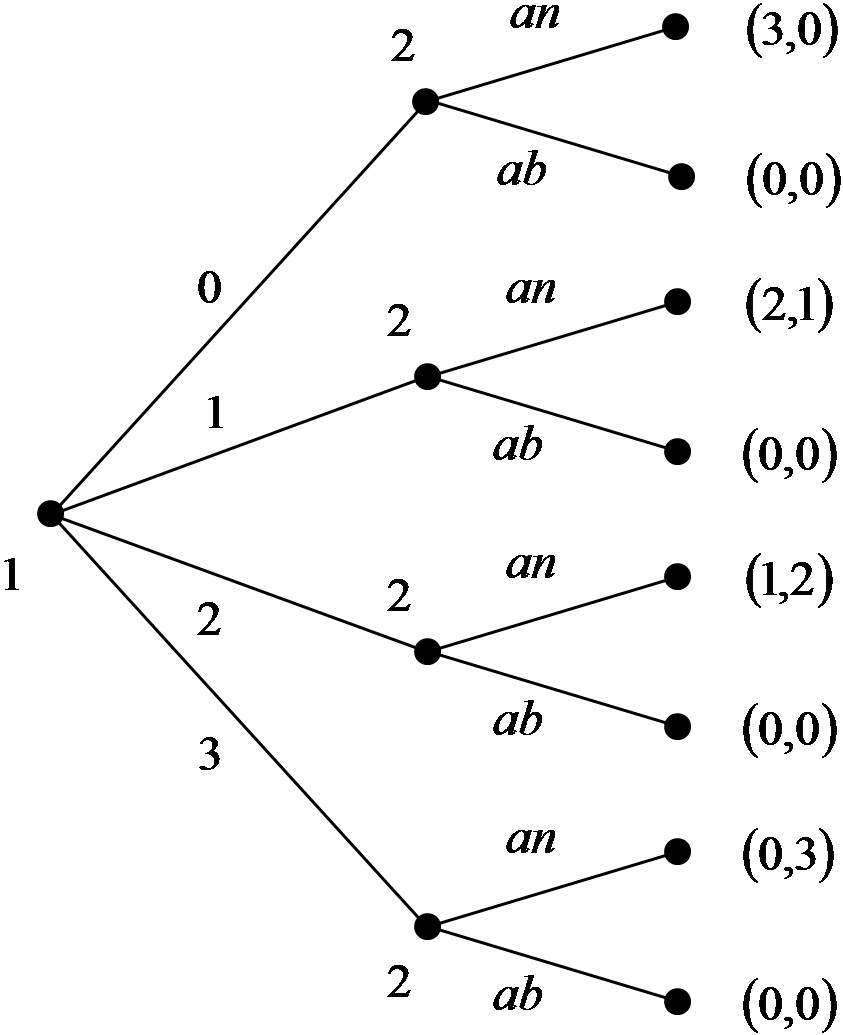
\includegraphics[width=100px]{./urbaum.png}
\end{center}

\textbf{eine} Strategie = eine Vorschrift, die an \textbf{jedem Knoten} eine Entscheidung festlegt;*vollständiger* Plan eines Spielers, was zu tun ist\\
Strategien Spieler 1: [0],[1],[2],[3]\\
Strategien Spieler 2: alle Reaktionen auf alle möglichen Angebote, \textbf{eine} beispielhafte Strategie = [0] annehmen, [1] annehmen, [2] ablehnen, [3] ablehnen

Menge der Strategien von S2 = 2\(^{\text{4}}\) (=16) also die eigenen Reaktionsmöglichkeiten (annehmen, ablehnen) hoch die Strategienanzahl von Spieler 1 (4), zB:
\begin{center}
\begin{tabular}{l}
(an, an, an, an)\\
(an, an, an, ab)\\
(an, an, ab, an)\\
(an, ab, an, an)\\
\ldots{}\\
\end{tabular}
\end{center}
Die strategische Form bildet all diese Strategien mit ihren Auszahlungen in einer Matrix ab
\begin{center}
\begin{tabular}{rllllll}
S1 $\backslash$ S2 & an,an,an,an & an,an,an,ab & an,an,ab,an & an,ab,an,an & \ldots{} & ab,ab,ab,ab\\
\hline
0 & (3,0) & (3,0) & (3,0) & (3,0) & \ldots{} & (0,0)\\
1 & (2,1) & (2,1) & (2,1) & (2,0) & \ldots{} & (0,0)\\
2 & (1,2) & (1,2) & (1,0) & (1,2) & \ldots{} & (0,0)\\
3 & (0,3) & (0,0) & (0,3) & (0,3) & \ldots{} & (0,0)\\
\end{tabular}
\end{center}
Hier ist ebenfalls die Rückwärtsinduktion beim Baum hilfreich um das Spiel zu lösen. Wenn man alle letzten Teilbäume betrachtet fällt schonmal auf das [ab,ab,ab,ab] also "ab" auf jedes Angebot nicht optimal ist \(\rightarrow\) kann somit gestrichen werden. Wiederholt man diesen Prozess des Vergleichens in der oberen Tabelle, verbleiben letztendlich nur noch [an,an,an,an] und [ab,an,an,an] als gleichwertig optimale Strategien fuer Spieler 2.\\
Spieler 1 braucht also nur noch diese beiden Strategien von Spieler 2 in Betracht ziehen und genau diese beiden Gleichgewichte sind auch teilspielperfekt. Ein teilspielperfektes Gleichgewicht ist ein NashGG das auch auf jedem Teilspiel ein NashGG ist.
\begin{center}
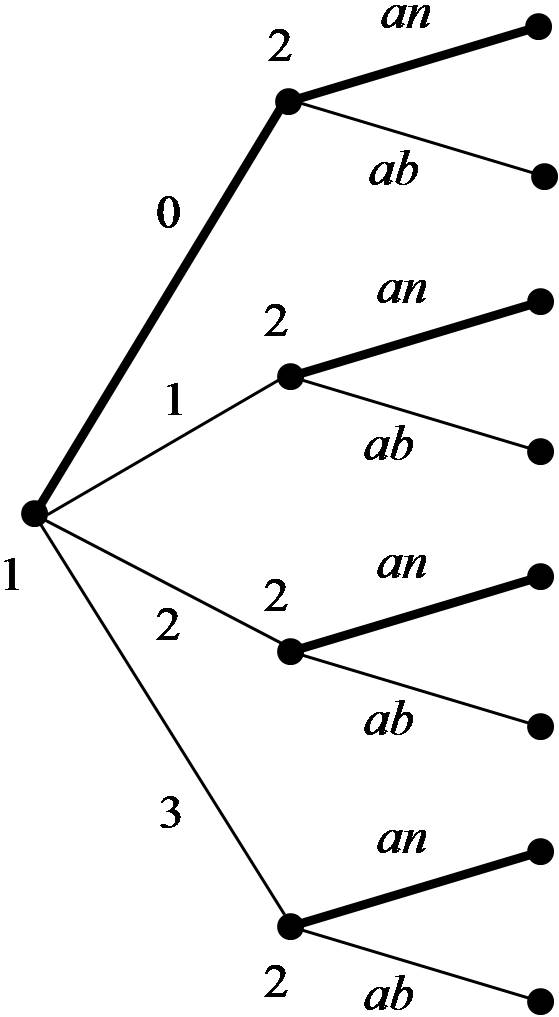
\includegraphics[height=0.4\textwidth]{./4an.png}
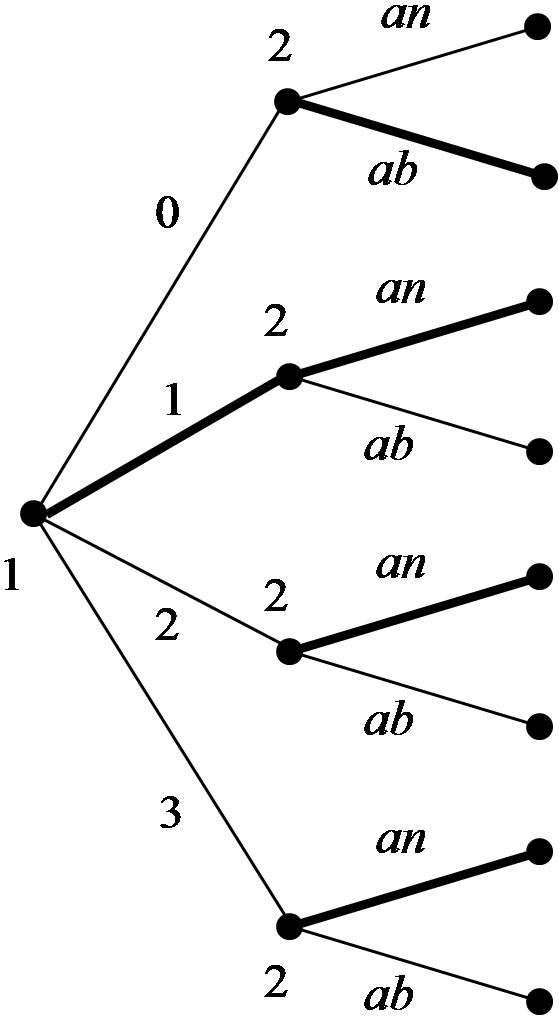
\includegraphics[height=0.4\textwidth]{./3an.png}
\end{center}

\subsection{Dynamische Spiele bei imperfekter Information}
\label{sec:org8f8c51a}
Züge der Natur sind ein möglicher Grund für imperfekte Information(möglicherweise asymmetrisch verteilte Information)
\(\rightarrow\) siehe F.120 / S.129
\paragraph{Bayes'sches Gleichgewicht}
Anfangs entsprechen die Informationsstände der Spieler den von der Natur vergegeben Wahrscheinlichkeiten.\\
Beispiel: Die Wahrsch. eines 1-Euro-“Typen” ist 50\%.
Aber bei längeren/dynamischen Spielen können Spieler durch ihre Entscheidungen ihren Typen (teilweise) offenbaren (zB Bieter bei einer offenen Auktion der seine eigene Zahlungsbereitschaft=Typ über die Gebote hinweg tlw. offenbart).\\
In einem \textbf{perfekten Bayes'schen Gleichgewicht}:
\begin{enumerate}
\item sind die Strategien der Spieler jederzeit optimal, gegeben die aktuellen Informationsstände
\item werden die Informationsstände jederzeit rational aktualisiert
\end{enumerate}
\end{document}
